\documentclass[a4paper,10pt]{article}
\title{CS 349 Assignment 2}
\author{Manan Gupta - 170101035}

\usepackage[shortlabels]{enumitem}
\usepackage[dvipsnames,table]{xcolor}
\usepackage[lmargin=1cm,rmargin=1cm,tmargin=0.5cm,bmargin=1.2cm]{geometry}
\usepackage{tabularx}
\usepackage{graphicx}
\usepackage{calc}
\usepackage{adjustbox}
\usepackage{lipsum}
\usepackage{wrapfig}
\usepackage{subfig}
\usepackage{textcomp}
\usepackage{sectsty}
\usepackage{hyperref}
\chapterfont{\color{blue}}  % sets colour of chapters
\sectionfont{\color{Fuchsia}} 
\newlength{\strutheight}
\settoheight{\strutheight}{\strut}

\makeatletter         
\renewcommand\maketitle{
	{\raggedright {
			\color{RoyalPurple}
		\begin{center}
			{\fontsize{22pt}{22pt} \bfseries \sffamily \@title } \qquad\qquad
			{\fontsize{22pt}{22pt} \bfseries \@author}\\[8ex]
\end{center}}} }
\makeatother
\begin{document}

\maketitle
\vspace{-1cm}
\hrule
\vspace{0.4cm}
\noindent
{\fontsize{18pt}{18pt} \bfseries \sffamily \color{RedViolet}\\Application Assigned : Hotstar Video Streaming\\
Link for data : \href{https://drive.google.com/drive/folders/14Bxr_9KKtqYI6y6nnKtwHtB8ZvGOMKf2?usp=sharing}{Drive Link}
}
\vspace{-0.3cm}
\section*{Question 1: Protocols Used}
\begin{enumerate}[{\color{Magenta}A)}]
	\item \textbf{\color{Magenta} \large Application Layer}
	\begin{itemize}
		\item \textbf{HTTP :} The protocol used in the application layer is \textbf{Hyper Text Transfer Protocol.} The HTTP messages are of two types, request and response. Request messages consist of a \textbf{request line}, followed by the \textbf{Header} and the \textbf{body} of the message. Response message format is similar but it has a \textbf{status line} instead of a request line. Request line holds the info regarding the \textbf{method} of the request, the server \textbf{URL} and the \textbf{version} of HTTP being used. Status line holds the \textbf{version}, the \textbf{status code}, and the status \textbf{phrase}. Header consists of \textbf{field name}-value pairs holding other meta information and finally the body consists of data that is sent or received.
		\begin{figure}[h]
			\centering
			\subfloat[HTTP Request Message]{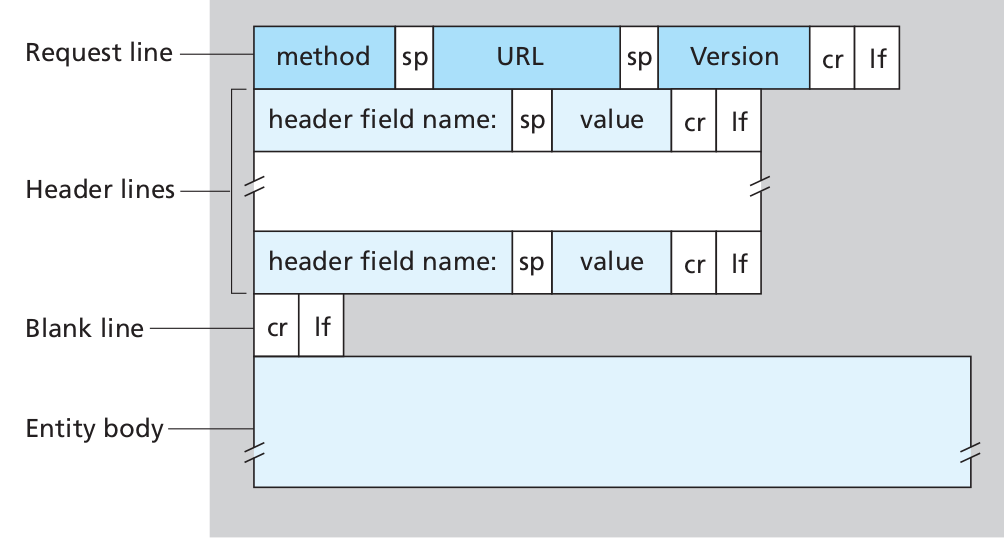
\includegraphics[width=0.5\textwidth]{Images/http_request}}
			\subfloat[HTTP Response Message]{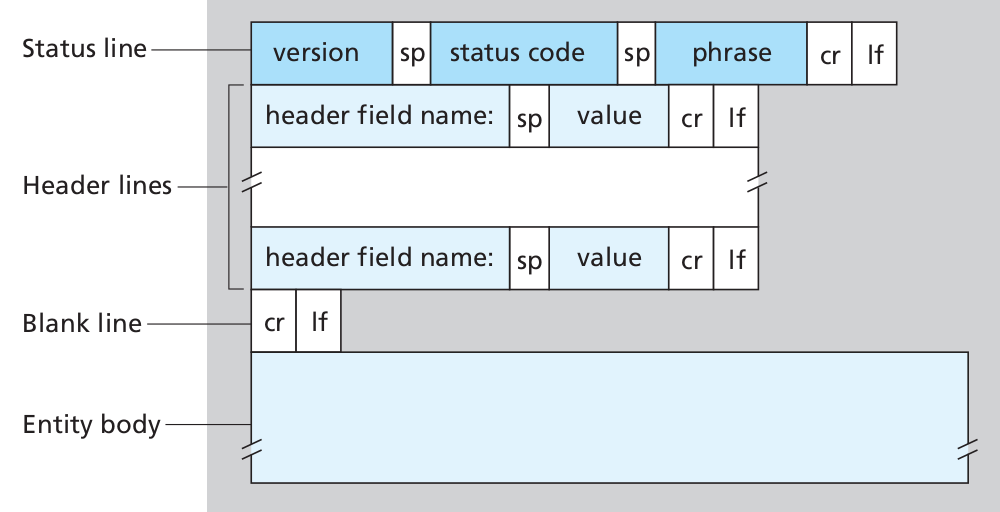
\includegraphics[width=0.5\textwidth]{Images/http_response}}
			\caption{HTTP Message Format}
		\end{figure}
		\vspace{-0.3cm}\item \textbf{TLSv1.2 :} TLSv1.2 is the successor of \textbf{SSL} and it provides communications security over a computer network. Symmetric cryptography is used to encrypt the data transmitted. The packet contains the type of message (handshake, alert, or data) in the '\textbf{Content Type}' field. It also contains the \textbf{version}, \textbf{length} of data and \textbf{MAC (Message Authentication Code)}.
		\begin{figure}[h]
			\centering
			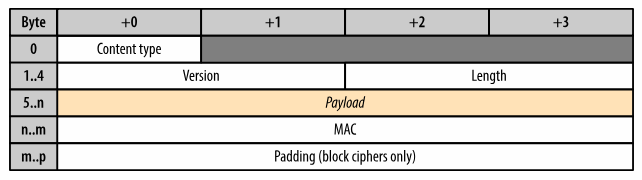
\includegraphics[width=0.7\textwidth]{Images/tls_message}
			\caption{TLSv1.2 Message Format}
		\end{figure}
	\end{itemize}
	\vspace{-0.3cm}\item \textbf{\color{Magenta} \large Transport Layer }\\
	\begin{adjustbox}{valign=T,raise=\strutheight,minipage={\linewidth}}
		\begin{wrapfigure}{r}{0pt}
			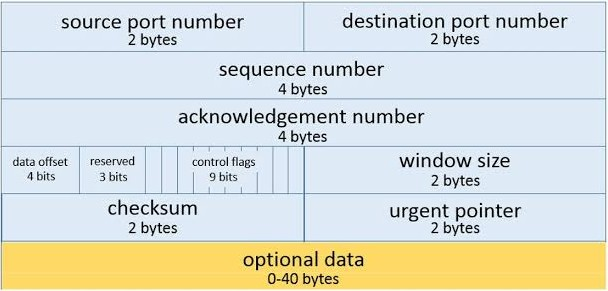
\includegraphics[width=10cm]{Images/tcp_segment}
			\caption{TCP Segment Format}
		\end{wrapfigure}
		\strut{}
		\textbf{Transmission Control Protocol} is a standard that defines how to establish and maintain a network conversation via which application programs can exchange data. \textbf{Source Port} and \textbf{Destionation Port} identify the hosts of the connection, source being the end point from where the segment is sent. \textbf{Sequence Number} specifies the number assigned to the first byte of data in the current message. If the ACK control bit is set, then \textbf{Acknowledgment number} refers to the next sequence number that the sender is expecting to receive. \textbf{Data offset} specifies the size of the variable-sized TCP header. \textbf{Flags} are 1 bit values that specify the state of the connection and are used for control. \textbf{Window size} is the size of the buffer of the receiver. \textbf{Checksum} is used for error correction. Data field contains the payload of the segment.
	\end{adjustbox} 
	\item \textbf{\color{Magenta} \large Network Layer }\\
	\begin{adjustbox}{valign=T,raise=\strutheight,minipage={\linewidth}}
		\begin{wrapfigure}{l}{0pt}
			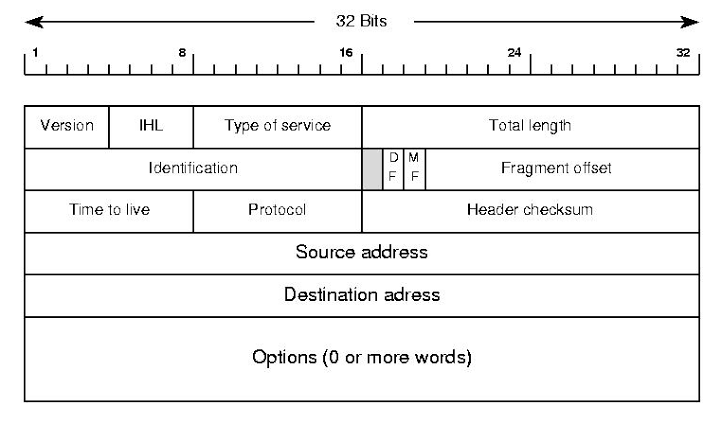
\includegraphics[width=10cm]{Images/ip_datagram}
			\caption{IP Datagram Header Format}
		\end{wrapfigure}
		\strut{}
		\textbf{IPv4 (Internet Protocol Version 4)} is one of the core protocols of standards-based internetworking methods in the Internet. It is used in packet-switched networks. Each IP datagram consists of a \textbf{header} and a \textbf{data} part. The header has a 20 byte fixed part followed by a variable-sized optional part. \textbf{Version} refers to the version of the datagram. In this case it would be 4. \textbf{IHL (Internet Header Length)} is the size of the header. \textbf{Types of Service} contains a 3-bit precedence field (that is ignored today), 4 service bits, and 1 unused bit. Service bits specify what characteristics the physical layer shhould use. \textbf{Total Length} is the total length of the datagram in bytes. \textbf{Identification} uniquely identifies the datagram. All fragments of a datagram contain the same identification value. \textbf{TTL (Time to Live)} is the maximum routers through which the segment can be switched. \textbf{Protocol} indicates the next higher level protocol that is contained within the data portion of the packet. \textbf{Header checksum} is used for error detection. \textbf{Source} and \textbf{destination addresses} are the addresses of the source and destination of the packet respectively.
	\end{adjustbox} 
	\item \textbf{\color{Magenta} \large Link Layer}\\
	\begin{adjustbox}{valign=T,raise=\strutheight,minipage={\linewidth}}
		\begin{wrapfigure}{r}{0pt}
			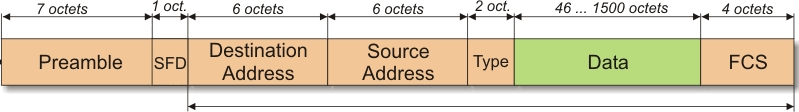
\includegraphics[width=12cm]{Images/ethernet_frame}
			\caption{Ethernet Frame Format}
		\end{wrapfigure}
		\strut{}
		\textbf{Ethernet II} is used in the link layer. \textbf{Preamble} is a 7-byte pattern of alternating 0's and 1's which indicates starting of the frame and allow the sender and receiver to establish bit synchronization. \textbf{SFD} is the start frame delimiter and marks the start of the frame. \textbf{Destination} and \textbf{source addresses} are the MAC addresses of the sending and receiving machines of the frame respectively. \textbf{Type} field is used to specify the protocol that is being used. \textbf{FCS (Frame Check Sequence)} is the error detecting code that is added. 
	\end{adjustbox} 
\end{enumerate}

\section*{Question 2: Observed Values in Different Protocols}
\begin{enumerate}[{\color{Magenta}A)}]
	\item \textbf{\color{Magenta} \large Application Layer}\\
	\begin{adjustbox}{valign=T,raise=\strutheight,minipage={\linewidth}}
		\begin{wrapfigure}{l}{0pt}
			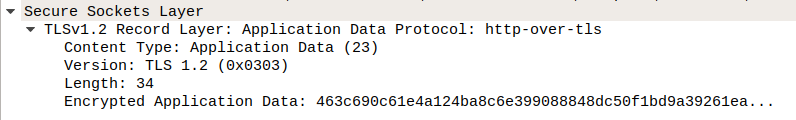
\includegraphics[width=10cm]{Images/AppEx}
			\caption{TLSv1.2 Record Example}
		\end{wrapfigure}
		\strut{}
		It is visible from the example that the application data protocol is \textbf{Http-over-tls} (aka HTTPS). The \textbf{content type} in this message is Application Data. \textbf{Version }of TLS is 1.2. \textbf{Length} of the data is 34 bytes. \textbf{Encrypted Application Data} can also be seen. 
		\\HTTPS encrypts all message contents, including the HTTP headers and the request/response data, therefore no HTTP header or request/response can be seen explicitly.
	\end{adjustbox}
	\item \textbf{\color{Magenta} \large Transport Layer }\\
	\begin{adjustbox}{valign=T,raise=\strutheight,minipage={\linewidth}}
		\begin{wrapfigure}{r}{0pt}
			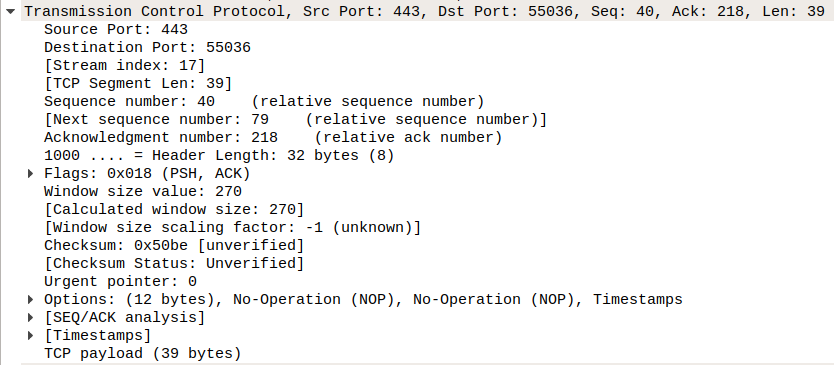
\includegraphics[width=10cm]{Images/TcpEx}
			\caption{TCP Segment Example}
		\end{wrapfigure}
		\strut{}
		It can be seen that the \textbf{source port} is 443 (This is to be expected because the default port for HTTPS connection is 443). The \textbf{destination port} is 55036. The \textbf{TCP Segment Length} is 39 bytes (payload). The \textbf{sequence number} is 40. \textbf{Acknowledgement number} is 218 which means that the sender of this segment is expecting a segment with sequence number 218 from the receiver. \textbf{Flags} field tells us that PSH and ACK flag is enabled. PSH flag is an option provided by TCP that allows the sending application to start sending the data even when the buffer is not full. \textbf{Window size} value is 270 (Number of packets sent before acknowledgment).	The \textbf{checksum} value can also be seen that is used for error detection.
	\end{adjustbox} 
	\pagebreak
	\item \textbf{\color{Magenta} \large Network Layer }\\
	\begin{adjustbox}{valign=T,raise=\strutheight,minipage={\linewidth}}
		\begin{wrapfigure}{l}{0pt}
			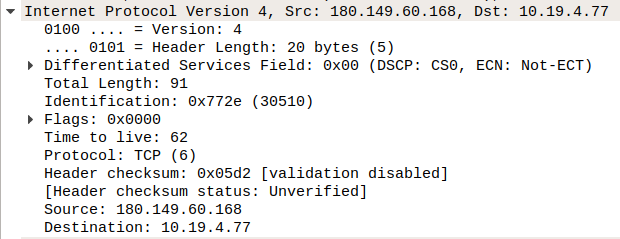
\includegraphics[width=10cm]{Images/IpEx}
			\caption{IP Datagram Example}
		\end{wrapfigure}
		\strut{}
		\textbf{Version}, as stated earlier, is 4 because IPv4 is being used. When IPv6 will be used, then the version will become 6. \textbf{Header Length} has the value 5 which implies that the header size is 20 bytes. \textbf{Total length} of the packet is 91 bytes and the \textbf{Identification number} is 0x772e. \textbf{Flag} value of 0000 implies that the datagram is not fragmented. \textbf{TTL} is 62 meaning that it can hop 62 times before dying. \textbf{Checksum} Value (0x05d2) can also be seen which is used for error detection. \textbf{Source address} (IP address of server) is 180.149.60.168. \textbf{Destination address} (IP address of my laptop) is 10.19.4.77
	\end{adjustbox} 
	\item \textbf{\color{Magenta} \large Link Layer }\\
	\begin{adjustbox}{valign=T,raise=\strutheight,minipage={\linewidth}}
		\begin{wrapfigure}{r}{0pt}
			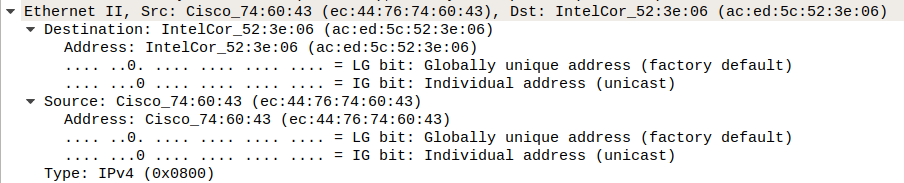
\includegraphics[width=12cm]{Images/linkEx}
			\caption{Ethernet Frame Example}
		\end{wrapfigure}
		\strut{}
		The information about the \textbf{Destination} and \textbf{Source MAC addresses} can be seen. They are unique addresses assigned to the \textbf{Network Interface controllers} of the machines. The source of this frame is a Cisco device and the destination is my laptop. The \textbf{Type} of connection can also be seen.
	\end{adjustbox} 
\end{enumerate}

\section*{Question 3: Protocols Used in Functioning of The Application}
\begin{enumerate}[{\color{Magenta}A)}]
	\item \textbf{\color{Magenta} \large Streaming}\\
	\begin{adjustbox}{valign=T,raise=\strutheight,minipage={\linewidth}}
		\begin{wrapfigure}{r}{0pt}
			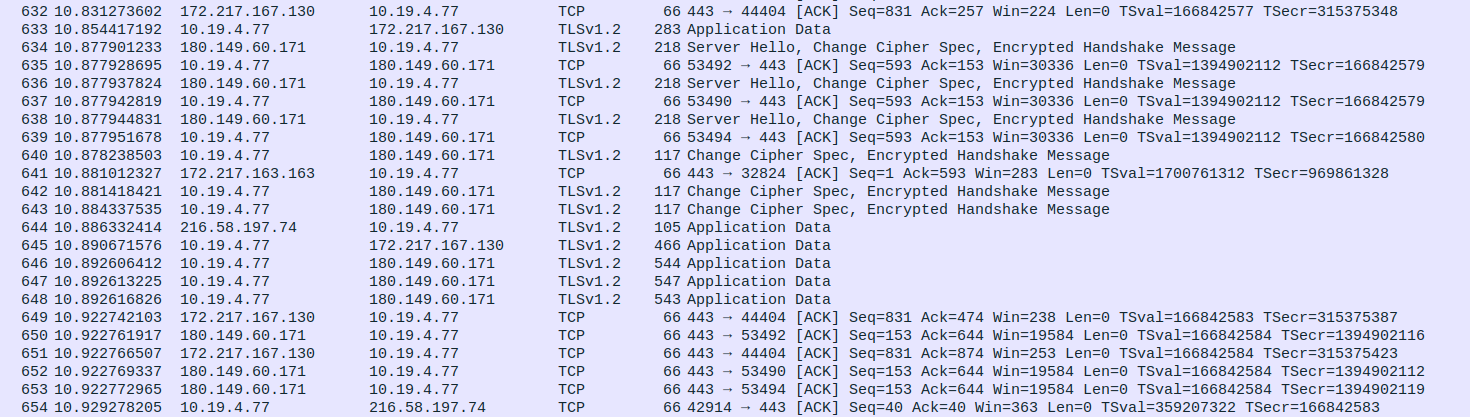
\includegraphics[width=14cm]{Images/stream}
			\caption{Example of Messages Transferred}
		\end{wrapfigure}
		\strut{}
		\textbf{HTTPS} (HTTP-over-TLS) is used in the Application Layer as HTTP is used by World Wide Web and defines how messages should be formatted and transmitted. \textbf{TLS} (Transport Layer Security) is a \textbf{cryptographic protocol} designed to provide communications \textbf{security} over a computer network. It \textbf{encrypts} the data and prevents hackers from \textbf{snooping}. It also prevents against \textbf{Man in the Middle} attacks. \textbf{TCP} is used at the Transport Layer as it is a \textbf{connection-oriented} \textbf{reliable} data transfer protocol. It offers facilities like \textbf{flow control}, \textbf{congestion control} and \textbf{error handling} mechanisms. Since the protocol is reliable, all the messages from the server reach the browser without any losses. This error-free connection is required by Hotstar because it offers very \textbf{high-quality streaming} (HD is also possible) which would not be possible otherwise. Also, the users can bo back and forth to different parts of a clip, unlike other live streaming services. IP protocol is used in the Network Layer as it is a requirement for using the Internet. IPv4 is a connectionless protocol for use on a packet-switched network. Ethernet(II) is used in the link-layer as it is one of the most widely used and reliable link layer protocol. It has \textbf{error handling} capabilities and ensures reliable data transfer between two network devices.
	\end{adjustbox} 
	\item \textbf{\color{Magenta} \large Pause}\\
	Just as the Pause button was pressed, a small number of packets were transmitted from the client to the server and vice versa. The content of these messages can however not be seen as TLS encrypts the message.
	\begin{figure}[h]
		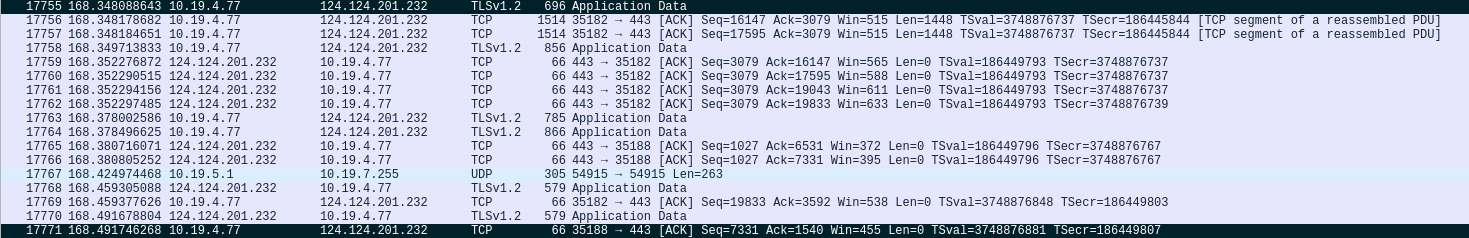
\includegraphics[width=\textwidth]{Images/pause1}
		\caption{Segments Transfered on Pause}
	\end{figure}

	\pagebreak
	Following this \textbf{Keep Alive} segments were sent from the client to the server telling the server \textbf{not to close} the TCP connection even though no data is being currently transferred. \textbf{Acknowledgment} for those Keep Alive messages can also be seen. These Keep Alive messages are very small in size and therefore do not use much bandwidth while the video is paused. \textbf{These segments are essential otherwise the connection would be closed and no further data could be transferred even if the video is unpaused.}
	\begin{figure}[h]
		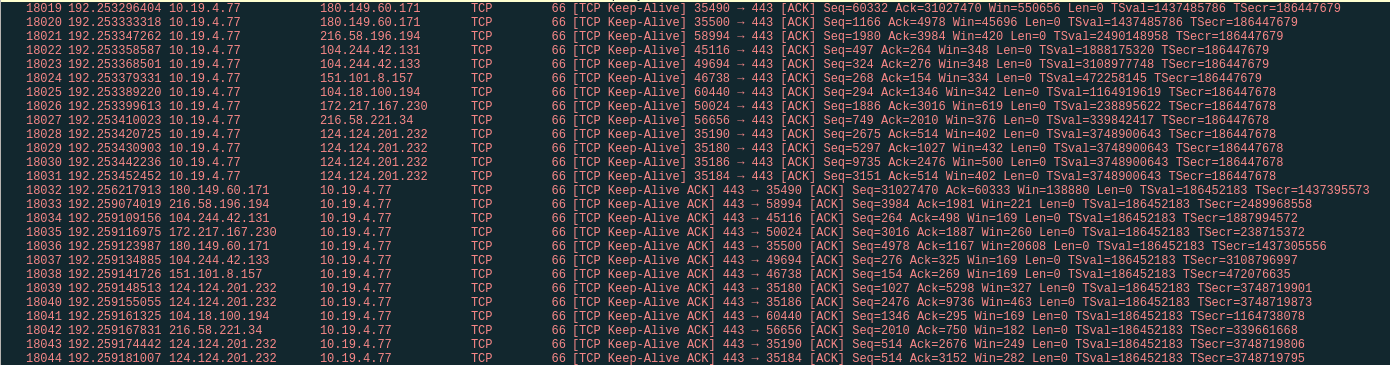
\includegraphics[width=\textwidth]{Images/pause2}
		\caption{Keep Alive Messages}
	\end{figure}
	\item \textbf{\color{Magenta} \large Play}\\
	Again a small number of segments are exchanged. Now the Keep Alive Messages stop though.
	\begin{figure}[h]
		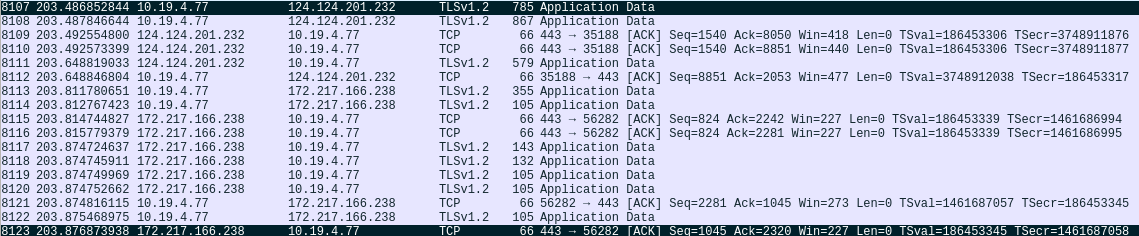
\includegraphics[width=\textwidth]{Images/play}
		\caption{ Segments Transfered on Play}
	\end{figure}
	\item \textbf{\color{Magenta} \large Skip 10 Seconds}\\
	Similar transfer of packets takes place between the client and the server.
\end{enumerate}
\section*{Question 4: Functionalities of the Application}
\begin{enumerate}[{\color{Magenta}A)}]
	\item \textbf{\color{Magenta} \large TCP Handshake}\\
	TCP connection is established via a \textbf{3 way handshake}. First the client sends a \textbf{SYN} segment to the server. The server responds with \textbf{ACK} for the request. It also sends a SYN in the same segment. Finally, the client responds with ACK and the connection is setup.
	\begin{figure}[h]
		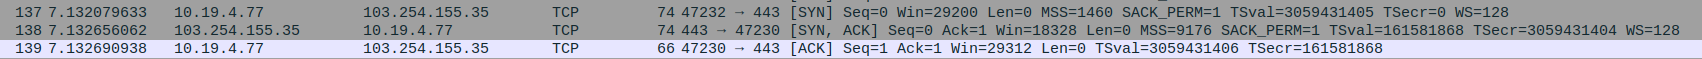
\includegraphics[width=\textwidth]{Images/TCP_handshake}
		\caption{TCP Handshake}
	\end{figure}
	\item \textbf{\color{Magenta} \large Application Layer Handshake}\\
	Before the client and the server can begin exchanging application data over TLS, the encrypted tunnel must be negotiated. The client and the server must agree on the version of the TLS protocol. They must choose the ciphersuite, and verify certificates if necessary.
	\\
	The first step of the handshake is \textbf{Client Hello}. Within this, the client sends a number of specifications in plain text, such as the version of the TLS protocol it is running, the list of supported \textbf{ciphersuites}, and other TLS options it may want to use.
	\\The second step is \textbf{Server Hello}. The server picks the TLS protocol version for further communication. It decides on a ciphersuite from the list provided by the client, attaches its certificate, and sends the response back to the client. Optionally, the server can also send a request for the client's certificate and parameters for other TLS extensions. 
	\\The third step is \textbf{Client and Server Key Exchange}. Assuming both sides are able to negotiate a common version and cipher, and the client is happy with the certificate provided by the server, the client initiates either the RSA or the Diffie-Hellman key exchange, which is used to establish the symmetric key for the ensuing session.
	\\The final step is \textbf{ChangeCipherSpec}. The server processes the key exchange parameters sent by the client, checks message integrity by verifying the MAC (Message Authentication Code), and returns an encrypted Finished message back to the client. On the client side, the message is decrypted with the negotiated symmetric key and the MAC is verified. If all is well, then the connection is established.
	\begin{figure}[h]
		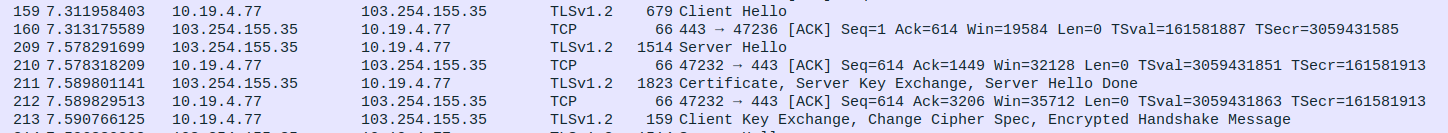
\includegraphics[width=\textwidth]{Images/TLS_handshake}
		\caption{TLS Handshake}
	\end{figure}
	\begin{figure}[h]
		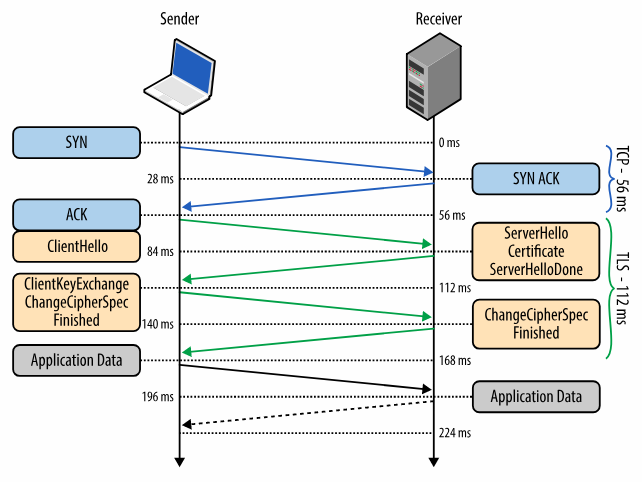
\includegraphics[width=\textwidth]{Images/Comp_pic}
		\caption{The Complete Picture}
	\end{figure}
	\item \textbf{\color{Magenta} \large Streaming}\\
	While streaming video, messsages are sent from the server to the client containg the information about the video. This can be seen in the image as TLS segments are labeled Application data. Some segments might be fragmented that are then joined again to form the complete message. Once the segments arrive, they are re-assembled and the payload is delivered to the application layer.
	\begin{figure}[h]
		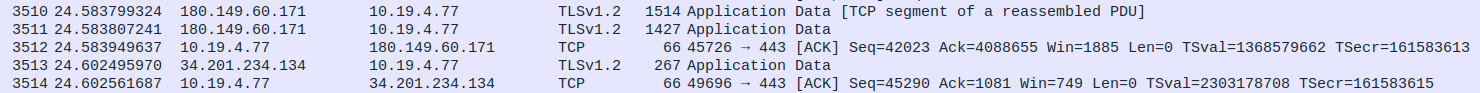
\includegraphics[width=\textwidth]{Images/stream2}
		\caption{Application Data Example}
	\end{figure}
	\item \textbf{\color{Magenta} \large Pause}\\
	The message transfered on pressing pause is shown below. A small number of segments are exchanged though their content cannot be understood as TLS encrypts them.
	\begin{figure}[h]
		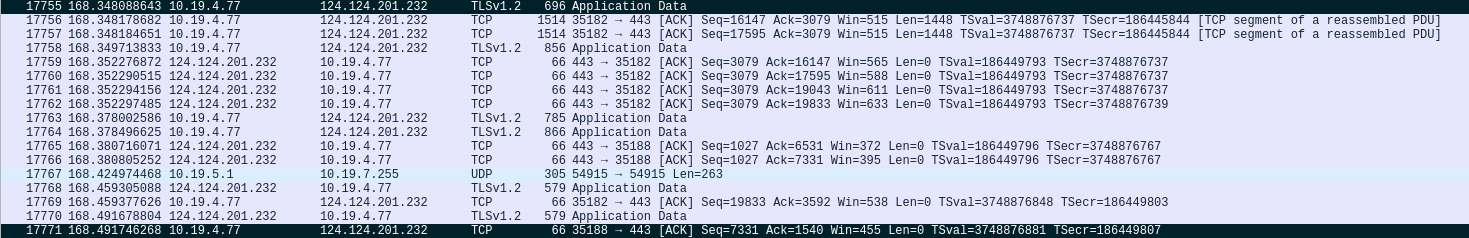
\includegraphics[width=\textwidth]{Images/pause1}
		\caption{Segments Transfered on Pause}
	\end{figure}
	\pagebreak
	\\
	\textbf{Keep Alive} segments are also sent from the client to the server as explained in the previous question. These segments and also their acknowledgments can be seen from the screenshot attached.
	\begin{figure}[h]
		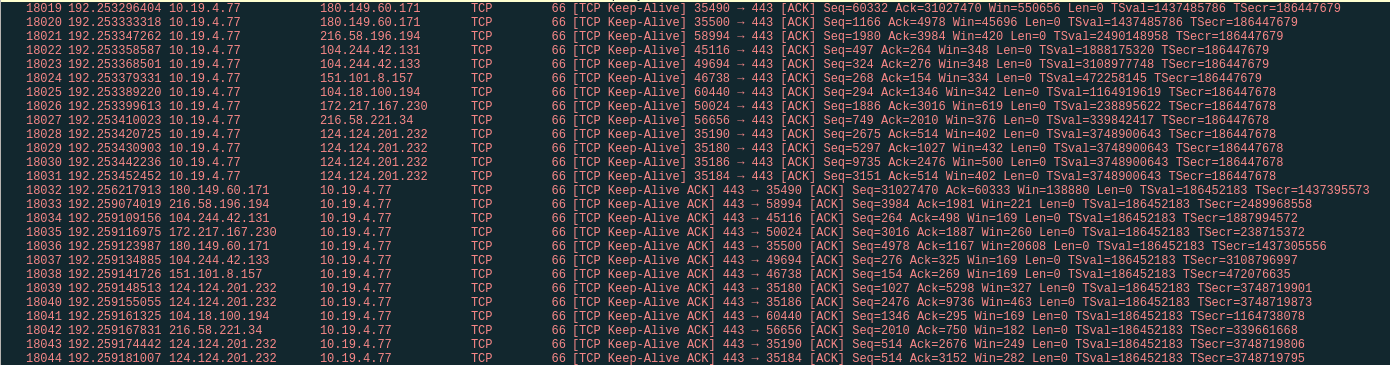
\includegraphics[width=\textwidth]{Images/pause2}
		\caption{Keep Alive Messages}
	\end{figure}
	\item \textbf{\color{Magenta} \large Play}\\
	Again a small number of segments are exchanged. Now the Keep Alive Messages stop though.
	\begin{figure}[h]
		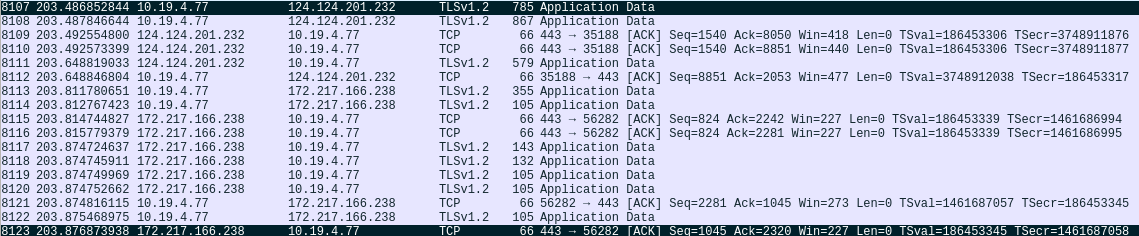
\includegraphics[width=\textwidth]{Images/play}
		\caption{Segments Transfered on Play}
	\end{figure}
	\item \textbf{\color{Magenta} \large TCP Connection Termination}\\
	\begin{adjustbox}{valign=T,raise=\strutheight,minipage={\linewidth}}
		The TCP connection termination phase uses a four-way handshake, with each side of the connection terminating independently. The client sends a FIN (piggybacked by an ACK) to the server which is ACKed by it. The server in turn sends a FIN which is ACKed by the client.
		\begin{wrapfigure}{r}{0pt}
			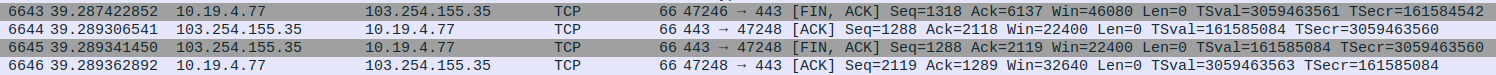
\includegraphics[width=\textwidth]{Images/TCP_end}
			\caption{TCP Connection Termination}
		\end{wrapfigure}
		\strut{}
	\end{adjustbox} 
\end{enumerate}
\pagebreak

\section*{Question 5: Statistical Analysis}
The data has been collected at 3 different times of the day:-
\begin{enumerate}[{\color{Magenta}1.}]
	\item \textbf{10:30 AM} in my room in Lohit using Mozilla Firefox web browser.
	\item \textbf{5:00 PM} in my room in Lohit using Mozilla Firefox web browser.
	\item \textbf{10:00 PM} in \textbf{Anchorenza and RadioG room} in New Sac using Mozilla Firefox web browser.
\end{enumerate}
\begin{table}[h]
	\rowcolors{1}{Magenta!10}{Magenta!20}
	\begin{tabularx}{\textwidth}{|p{220pt}||X||X||X|}
		\hline
		\rowcolor{Magenta!40}
		\textbf{Statistic Name} & \textbf{10:30 (Room)} & \textbf{17:00 (Room)} & \textbf{22:00 (New Sac)} \\ \hline
		\textbf{Throughput}  & 38795.027 Bytes/sec & 217567.01 Bytes/sec & 994580.82 Bytes/sec \\ \hline
		\textbf{RTT}  & 40.56 ms & 9.52 ms & 0.2 ms \\ \hline
		\textbf{Packet Size} & 1171.67 Bytes & 1221.18 Bytes & 1433.02 Bytes \\ \hline
		\textbf{Number of Packets Lost}  & 0 & 0 & 0\\ \hline
		\textbf{Number of UDP Packets} & 950 & 794 & 2180 \\ \hline
		\textbf{Number of TCP Packets}& 9476 & 29635 & 41782\\ \hline
		\textbf{Number of Responses Received per Request}& 6138/3511 (1.74) & 19530/10446 (1.87) & 26376/15475 (1.70)\\ \hline
	\end{tabularx}
	\caption{Statistical Ananlysis at 3 Different Times}
\end{table}
Although Hotsar does not use UDP at the transport layer, UDP packets are still observed. The reason is that DNS uses UDP packets and DNS resolution is an integral part of running any web application to find its servers IP address from the given hostname.

\section*{Question 6: Multiple Sources}
The data arrived from many different IP addresses. A few of which have been listed below.
\begin{itemize}[{\color{Magenta}$\star$}]
	\item \textbf{180.149.60.171}
	\item \textbf{180.149.60.168}
	\item \textbf{180.149.60.139}
	\item \textbf{124.124.201.232}
	\item \textbf{172.217.166.238}
	\item \textbf{103.254.155.35}
\end{itemize}
\begin{adjustbox}{valign=T,raise=\strutheight,minipage={\linewidth}}
	\begin{wrapfigure}{r}{0pt}
		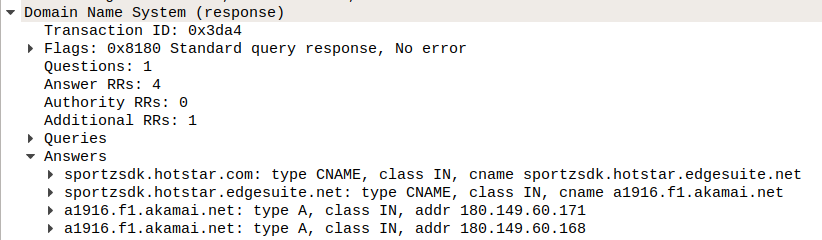
\includegraphics[width=12cm]{Images/DNS_response}
		\caption{DNS Response}
	\end{wrapfigure}
	\strut{}
	
	Most of the data arrived from the first 2 addresses. It can be seen from the attached screenshot that the canonical name for hotstar is \textbf{cname.hotstar.edgesuite.net} and the two servers are actually \textbf{Akamai} servers. Akamai is the leading \textbf{Content Delivery Network} (CDN) services provider for media and software delivery. So we can conclude that hotstar uses Akamai's services for content delivery. \\
	Data is sent from multiple servers because it leads to \textbf{Load Balancing}. Data comes through different paths so there is less network congestion and lesser load on each individual server. Multiple servers also lead to increased reliability as there is \textbf{no single point of failure}. Even if one server crashes, the service does not stop.
\end{adjustbox} 
\end{document} 
